\chapter{The three operations: maths in plain language}\label{ch:math}

\section{RGB to gray}

\subsection{The idea}

Gray is a weighted average of red, green and blue. The weights are not equal because the human eye is most sensitive to green and least to blue. The standard (ITU-R BT.601) weights are
\[
Y = 0.299\,R + 0.587\,G + 0.114\,B .
\]
A pure green pixel therefore looks much brighter in gray than a pure blue one of the same intensity.

\subsection{Doing it with integers only}

Floating-point is not needed, and integer arithmetic is easier to make exact and fast. Multiply the three weights by 256 and round: $0.299\cdot256=76.5\to77$, $0.587\cdot256=150.3\to150$, $0.114\cdot256=29.2\to29$. These add up to exactly $256$, so a white pixel stays white ($255\cdot256/256=255$). Dividing by 256 is the same as shifting right by 8 bits:
\begin{equation}
Y=\Big\lfloor\frac{77R+150G+29B+128}{256}\Big\rfloor=(77R+150G+29B+128)\gg 8 .
\end{equation}
The ``$+128$'' is half of 256: it turns the floor (rounding down) into rounding to the nearest integer. The coefficients are the ones JPEG-style converters use; the quick check is
\[
R=255,G=0,B=0\;\Rightarrow\;(77\cdot255+128)\gg8=19\,763\gg8=77,\qquad
R=G=B=255\;\Rightarrow\;(65\,280+128)\gg 8=255 .
\]

\begin{plain}
\textbf{Why this matters for SIMD.} The largest possible intermediate value is $77\cdot255+150\cdot255+29\cdot255+128=65\,408$, which is smaller than $2^{16}=65\,536$. So the whole computation fits in \emph{unsigned 16-bit} numbers and a 256-bit register can hold 16 of them at once. The test \code{gray\_exhaustive\_all\_16777216\_colours} runs every one of the $256^3$ colours through every implementation: a proof by exhaustion, not a sample.
\end{plain}

\section{2D convolution}

\subsection{The idea}

A \emph{kernel} is a small grid of weights, for example $3\times3$. To filter an image, slide the kernel over every pixel; at each position multiply the weights with the pixels underneath, add up, and write the sum to the output pixel.

\begin{center}
\begin{tikzpicture}[x=0.55cm,y=0.55cm,font=\scriptsize]
\foreach \x in {0,...,6}\foreach \y in {0,...,5}{ \node[draw=gray!50,minimum size=0.55cm,inner sep=0] at (\x,-\y) {}; }
\foreach \x in {2,3,4}\foreach \y in {1,2,3}{ \node[draw=accent,fill=plainbg,minimum size=0.55cm,inner sep=0] at (\x,-\y) {}; }
\node[draw=warnfg,fill=warnbg,minimum size=0.55cm,inner sep=0] at (3,-2) {\textbf{p}};
\node at (3,-5.9) {input image};
\begin{scope}[xshift=5.1cm]
\foreach \x/\y/\v in {0/0/w_{00},1/0/w_{01},2/0/w_{02},0/1/w_{10},1/1/w_{11},2/1/w_{12},0/2/w_{20},1/2/w_{21},2/2/w_{22}}{
 \node[draw=accent,fill=plainbg,minimum size=0.75cm,inner sep=0] at (\x*0.75,-\y*0.75-1) {$\v$}; }
\node at (0.75,-3.6) {kernel $w$};
\end{scope}
\draw[-{Stealth},thick] (8.2,-2.0) -- (9.2,-2.0);
\begin{scope}[xshift=10.2cm]
\foreach \x in {0,...,2}\foreach \y in {0,...,2}{ \node[draw=gray!50,minimum size=0.55cm,inner sep=0] at (\x,-\y-1) {}; }
\node[draw=warnfg,fill=warnbg,minimum size=0.55cm,inner sep=0] at (1,-2) {$p'$};
\node at (1,-4.4) {output pixel};
\end{scope}
\end{tikzpicture}
\end{center}

In formulas, for a kernel of size $k=2r+1$:
\begin{equation}
\text{out}(x,y)=\operatorname{clamp}\Big(\operatorname{round}\Big(\sum_{j=0}^{k-1}\sum_{i=0}^{k-1} w_{ji}\;\text{in}(x+i-r,\;y+j-r)\Big),\,0,\,255\Big).
\end{equation}
Each output pixel costs $k^2$ multiplications and $k^2$ additions: $3\times3$ is 9, $9\times9$ is 81, $31\times31$ is 961. That cost growth is why convolution is the classic target for optimization.

\begin{warn}[``Convolution'' versus ``correlation'']
Mathematically, convolution flips the kernel before sliding it; the operation above, without the flip, is called \emph{correlation}. Image libraries (OpenCV's \code{filter2D}, for example) implement the unflipped version and call it convolution. For kernels that are symmetric the two are identical; for an asymmetric kernel such as \emph{emboss} the result is mirrored. If an interviewer asks, say which one you implemented: correlation, same as OpenCV.
\end{warn}

\subsection{Kernels you can try}

\begin{center}
\small
\begin{tabular}{@{}lcp{9cm}@{}}
\toprule
\textbf{name} & \textbf{kernel} & \textbf{effect}\\ \midrule
box (blur) & $\tfrac19\begin{psmallmatrix}1&1&1\\1&1&1\\1&1&1\end{psmallmatrix}$ & each pixel becomes the average of its neighbourhood: smooths noise, loses detail.\\
binomial & $\tfrac1{16}\begin{psmallmatrix}1&2&1\\2&4&2\\1&2&1\end{psmallmatrix}$ & a blur that weights the centre more; the weights are exact binary fractions, which makes it perfect for tests (Chapter~\ref{ch:testing}).\\
Gaussian & bell-shaped weights, $\sigma$ sets width & the ``natural'' blur; the larger $\sigma$ (and $k$), the stronger.\\
sharpen & $\begin{psmallmatrix}0&-1&0\\-1&5&-1\\0&-1&0\end{psmallmatrix}$ & centre minus neighbours added back: exaggerates edges. Weights sum to 1, so overall brightness is unchanged.\\
identity & a single 1 in the middle & output equals input (a test).\\ \bottomrule
\end{tabular}
\end{center}

\begin{center}
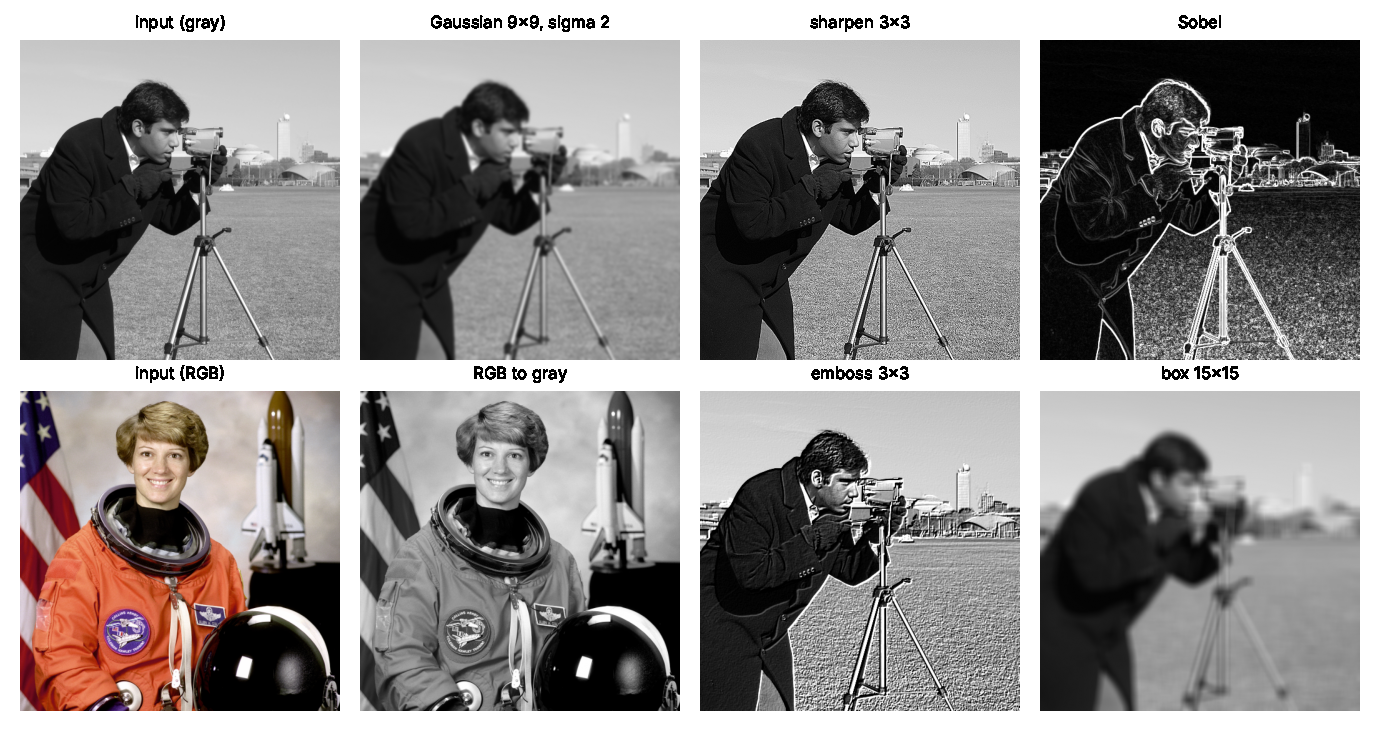
\includegraphics[width=\textwidth]{figures/f_ops_gallery.pdf}
\captionof{figure}{The operations on the standard ``cameraman'' photograph and on a colour image. Produced by the command line tool.}
\end{center}

\section{Sobel edge detection}

\subsection{The idea}

An edge is a place where brightness changes quickly. The change of brightness in a direction is a \emph{derivative}; for pixels it is the difference of neighbours. The simplest horizontal difference is $\text{in}(x+1)-\text{in}(x-1)$. Differences amplify noise, so Sobel first \emph{smooths} across the other direction using weights $1,2,1$ and only then differences:
\[
G_x=\begin{pmatrix}-1&0&1\\-2&0&2\\-1&0&1\end{pmatrix}\!*\text{in}
=\underbrace{\begin{pmatrix}1\\2\\1\end{pmatrix}}_{\text{smooth vertically}}\!\!\cdot\underbrace{\begin{pmatrix}-1&0&1\end{pmatrix}}_{\text{difference horizontally}}\!*\text{in},\qquad
G_y=\begin{pmatrix}-1&-2&-1\\0&0&0\\1&2&1\end{pmatrix}\!*\text{in}.
\]
$G_x$ responds to vertical edges, $G_y$ to horizontal edges. The edge strength combines both:
\begin{equation}
\text{out}=\min\!\big(255,\;|G_x|+|G_y|\big)\qquad\text{(the exact length would be }\sqrt{G_x^2+G_y^2}\text{)}.
\end{equation}
We use $|G_x|+|G_y|$, the common ``L1'' shortcut: it needs no square root, so it stays in integers and in 16-bit lanes. It overestimates the true length for diagonal edges by at most a factor $\sqrt2$, which is irrelevant for a detector that is thresholded afterwards, but you should know that it is an approximation.

\begin{center}
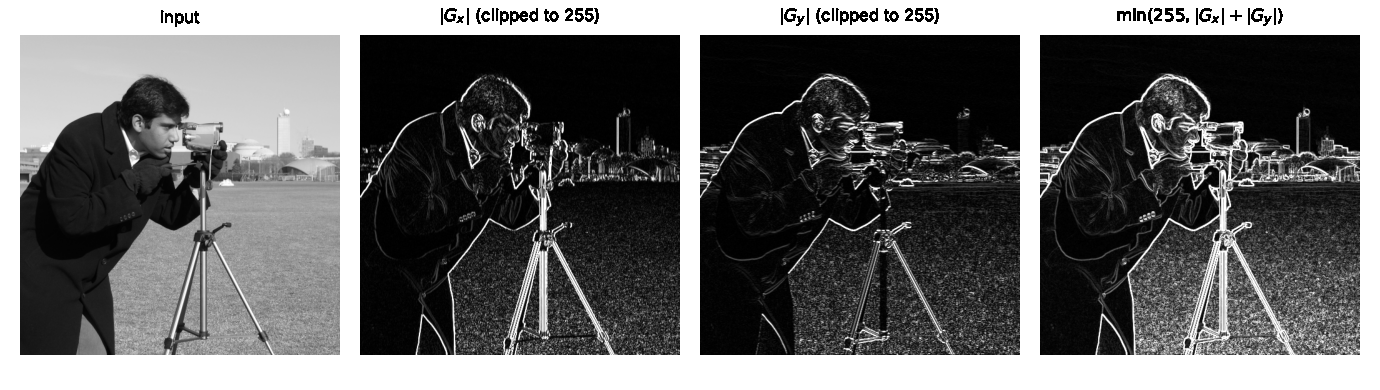
\includegraphics[width=\textwidth]{figures/f_sobel_parts.pdf}
\captionof{figure}{Left to right: the photograph, $|G_x|$ (vertical edges), $|G_y|$ (horizontal edges), and the final edge strength $\min(255,|G_x|+|G_y|)$.}
\end{center}

\subsection{How big can the numbers get? (this decides the data type)}

Each of $G_x$, $G_y$ is a sum of weights $\{1,2,1\}$ times pixels in $[0,255]$ with the positive and negative halves separated. The worst case is $4\cdot255=1020$ in magnitude, so $|G_x|+|G_y|\le2040<32\,768$. Everything fits in \textbf{signed 16-bit} integers (16 per 256-bit register) with no overflow: no wider type is needed, so no speed is wasted. Only the last step needs care: values above 255 must be clamped when converting back to 8 bits, which the instruction \code{packus} does for free (Chapter~\ref{ch:sobel}).

\begin{sound}
``Gray uses the 77/150/29 fixed-point weights, exact in 16-bit unsigned arithmetic, and I proved it for all 16.7 million colours. Sobel is the separable $[1\,2\,1]\otimes[-1\,0\,1]$ pair with an L1 magnitude, which stays within 16-bit signed lanes. Convolution is a $k\times k$ correlation in float32 with replicated borders and round-to-nearest-even output.''
\end{sound}
